%%%%% Physik Kompendium Nr.2 %%%%%
%% 06 -- Der Siebkreis %%

Der Siebkreis ist eine bekannte technische Anwendung, deren Schaltung aus den drei Wechselstromwiderstandstypen besteht (Häufig R-C-L-Schaltung genannt).
Ihre Aufgabe ist es, einen bestimmten, recht schmalen Frequenzbereich \glqq herauszufiltern\grqq , will sagen, dort die geringste Impedanz aufzuweisen.

Die Komponenten sind alle in Reihe geschaltet und der Widerstand kann in der Praxis weggelassen werden, da eine reelle Spule immer auch einen Ohm'schen Widerstand aufweist (sie besteht aus Draht). Da in der Theorie eine Spule immer als ideale Spule, also ohne sonstigen Widerstand, wird er in diesen Betrachtungen immer gesondert bezeichnet.

\begin{figure}[h!]
	\centering
	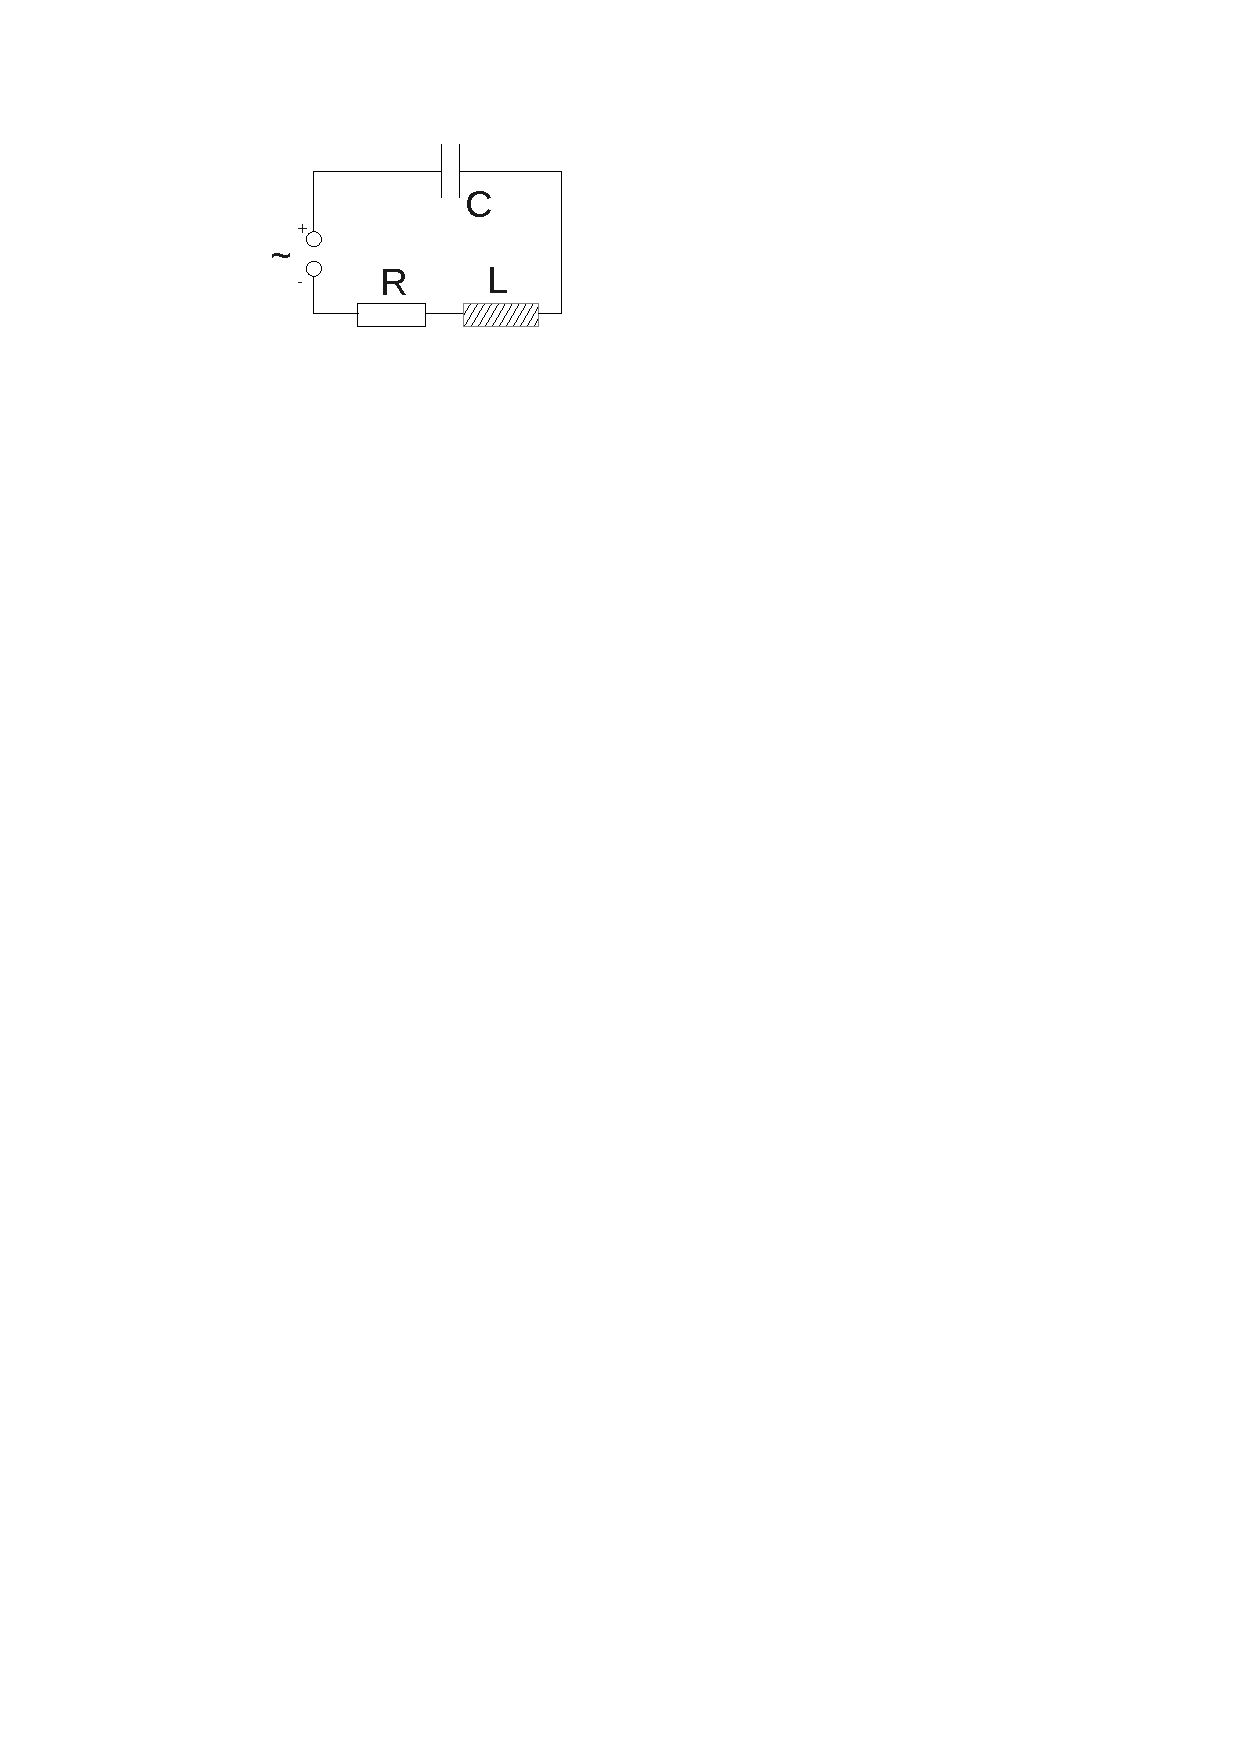
\includegraphics[width=0.5\textwidth]{Pictures/Siebkreis}
	\caption{Diagramm der Schaltung}
\end{figure}

Der Kondensator \glqq schneidet\grqq{} die hohen Frequenzen \glqq ab\grqq , die Spule die tiefen. Siehe Sektionen \ref{subsec:Frequenzabhaengigkeit} und \ref{subsec:AuswirkungenWiderstand}

Der Frequenzbereich wird durch die Daten der Bauteile bestimmt. 

\subsection{Resonanzfrequenz berechnen}

Die Resonanzfrequenz ist die Frequenz, bei der die Impedanz so klein wie möglich ist, d.h. die angestrebte Frequenz, die herausgefiltert werden soll.

Um eine kleinstmögliche Impedanz zu erreichen, muss der Blindwiderstand $=0$ sein. Aus Gleichung \ref{eq:BlindwiderstandSumme} abgeleitet, gilt:

\begin{align}	\label{eq:Resonanzfrequenz}
\begin{split}
	X_L - X_C &= 0 \\
	X_L &= X_C \\
	\omega \cdot L &= \frac{1}{\omega \cdot C} \\
%	\omega ^2 &= \frac{1}{C \cdot L} \\
	\omega &= \frac{1}{\sqrt{C \cdot L}} \\	
	f &= \frac{1}{2 \pi \cdot \sqrt{C \cdot L}} \\
\end{split}
\end{align}